\section{Results}
\label{sec:replication-results}

\subsection{RQ1: Time-Sensitive Validation}

In this research question, we compare prediction model performance using a time-sensitive validation and a classical validation.

Figures~\ref{fig:prec-java}-\ref{fig:mcc-java} show the performance of our Random Forest classifier under time-sensitive and classical validation. 
Overall, we observe that the validation setup has an impact on the classifier performance.
This impact varies significantly depending on the project, its size, and history of flaky tests.
The projects Achilles, Hbase, OkHttp, and Togglz observe a decrease in their MCC score.
The largest performance drop is observed in the OkHttp project, where the MCC dropped from 0.39 to 0.18.
The two exceptions are for Oozie and Oryx, where MCC increased by 0.10 and 0.13 points respectively. 
In the case of Oryx, this can be explained by the fact that most of the flaky tests come from one revision, thus, the time-sensitive validation has little to no impact. 
The difference can then be explained by the random selection of the samples when splitting the training and test set. 
The phenomenon is only present for this project.
In the case of Oozie, there is a considerable imbalance between the number of flaky tests (1039) and non-flaky tests (44). 
Hence, the test set contains only 9 non-flaky tests, which might not be enough to draw conclusions.\\

\begin{tcolorbox}[
    left=2pt,right=2pt,top=2pt,bottom=2pt,
    arc=0pt,
    boxrule=1.2pt
]
\textbf{RQ1:} The performances of a vocabulary-based model decrease under a time-sensitive validation (MCC value drops up to 0.21).
Nonetheless, the approach is still able to decently predict flaky tests.
\end{tcolorbox}

\begin{figure}
  \centering
  \begin{minipage}[b]{0.4\textwidth}
    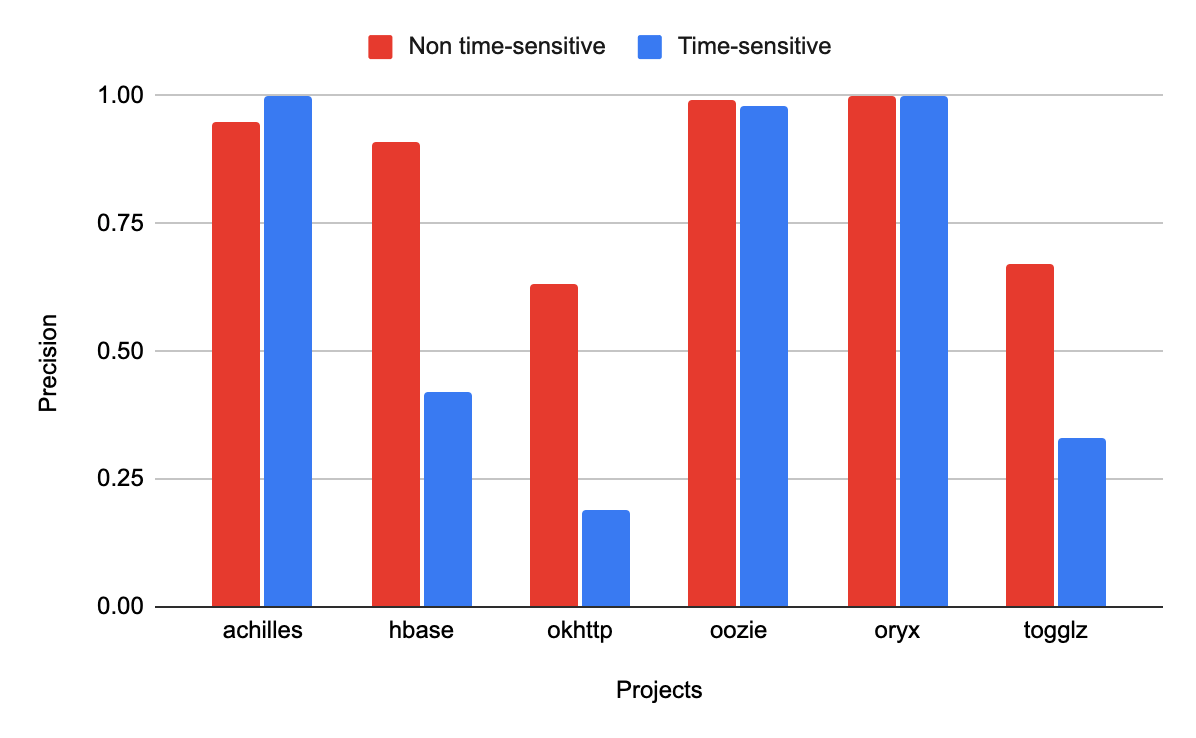
\includegraphics[width=\textwidth]{figures/replication/RQ1JavaPrecision.png}
    \caption{Precision under classical and time-sensitive validations.}
    \label{fig:prec-java}
  \end{minipage}
  \hfill
  \begin{minipage}[b]{0.4\textwidth}
    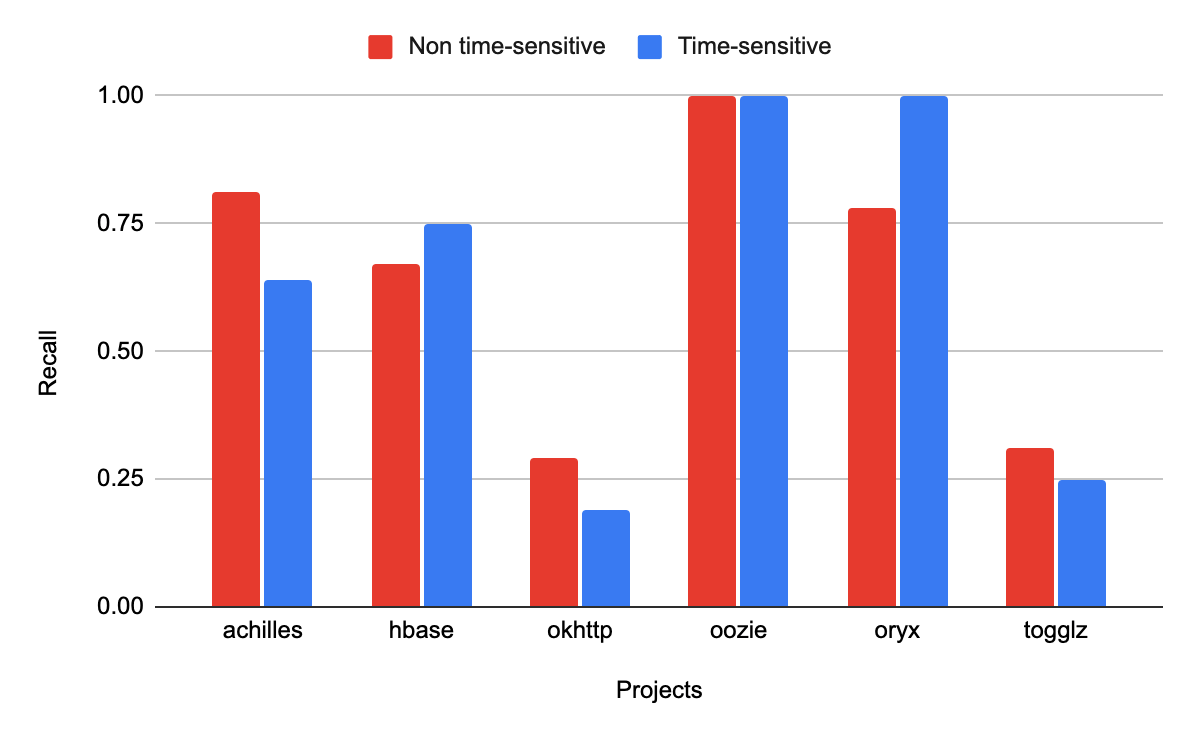
\includegraphics[width=\textwidth]{figures/replication/RQ1JavaRecall.png}
    \caption{Recall under classical and time-sensitive validations.}
    \label{fig:recall-java}
  \end{minipage}
  \hfill
  \begin{minipage}[b]{0.4\textwidth}
    \includegraphics[width=\textwidth]{figures/replication/RQ1JavaMcc.png}
    \caption{MCC under classical and time-sensitive validations.}
    \label{fig:mcc-java}
  \end{minipage}
\end{figure}

\subsection{RQ2: Generalisation to other Programming Languages}
\subsubsection{Predicting flaky tests in Python}
Table~\ref{python} reports on the model performance when predicting flaky tests in 9 Python projects. 

\begin{table}[t]
\centering
\caption{Classifier performance for Python projects}
\label{python}
 \begin{tabular}{l|r r r r r} 
 \toprule
 \textbf{Project} & \textbf{Precision} & \textbf{Recall} & \textbf{F1} & \textbf{MCC} & \textbf{AUC} \\ [0.25ex]
 \midrule
 bokeh & \textbf{1.00} & \textbf{0.91} & \textbf{0.95} & \textbf{0.95} & \textbf{0.95} \\
 cassandra-dtest & \textbf{0.96} & 0.43 & 0.58 & 0.63 & 0.71 \\
 celery & 0.85 & 0.54 & 0.64 & 0.66 & 0.77 \\
 jira & \textbf{0.98} & \textbf{0.99} & \textbf{0.99} & \textbf{0.95} & \textbf{0.98} \\
 pipenv & 0.78 & 0.19 & 0.30 & 0.37 & 0.60 \\ 
 python-amazon & \textbf{0.97} & \textbf{1.00} & \textbf{0.99} & \textbf{0.95} & \textbf{0.96} \\ 
 python-telegram-bot & \textbf{1.00} & \textbf{0.99} & \textbf{1.00} & \textbf{0.99} & \textbf{1.00} \\ 
 spyder & \textbf{0.92} & 0.77 & 0.83 & 0.82 & 0.88 \\ 
 typed-python & \textbf{1.00} & 0.86 & \textbf{0.91} & \textbf{0.92} & \textbf{0.93} \\ 
 \bottomrule
\end{tabular}
\end{table}

First, we observe that for 5 projects out of 9, the model reaches a great performance with MCC values greater than 0.9. 
For the rest of the projects, these scores are always higher than 0.50, except for Pipenv, which shows the lowest results with an MCC value of 0.37.
Similarly, all the studied projects have a F1-score greater than 90\% and 7 out of the 9 studied projects have a precision higher than 60\%.
These observations show that the vocabulary-based model is able to predict flaky tests with decent performance in Python projects.

\subsubsection{Predicting manifest flaky tests}

Table \ref{pythonManifestResults} shows the model performance in detecting manifest flaky tests based on tests marked as flaky by developers.
The results show a perfect performance with MCC and F1-score values of 1 and 100\% respectively, confirming that a model trained on tests labelled by developers can be used to predict manifest flaky tests.
Interestingly, 2 of the 20 manifest tests were not labelled as flaky by the developers and were only identified with the reruns.
Yet, the model was able to predict them by only learning from tests marked by developers.
In a real-world scenario, we could picture the model finding those tests and automatically annotating them.

\begin{table}[t!]
\caption{Classifier performance for manifest flaky test in the Python-telegram-bot project}
\label{pythonManifestResults}
\centering
 \begin{tabular}{l|r r r r r} 
 \toprule
 \textbf{Project} & \textbf{Precision} & \textbf{Recall} & \textbf{F1} & \textbf{MCC} & \textbf{AUC} \\ [0.25ex]
 \midrule
 python-telegram-bot & 1.00 & 1.00 & 1.00 & 1.00 & 1.00 \\ 
 \bottomrule
\end{tabular}
\end{table}

Figure \ref{manifest-flaky-example} shows the test \texttt{test\_idle()} from the class \texttt{TestUpdater}\footnote{https://github.com/python-telegram-bot/python-telegram-bot}.
Over 300 reruns, this test failed intermittently because of a concurrency issue where a scheduler has been shut down. 
Indeed, the test body contains several keywords related to time and concurrency, which are common causes of flakiness, \eg \texttt{Thread, sleep, idle}. 
In order to understand how the model predicted that this test is flaky, we analyse the most important features of the model. 
These features do not completely reflect the model prediction and they can be biased~\cite{Permutat82:online}, but they give us an idea of the vocabulary that the classifier is using for its predictions.
In the project Python-telegram-bot, we found that the top ten features include the keywords: \texttt{process, timeout, duration, seconds}, which are also related to time and concurrency.
Hence, the model's ability to predict the test flakiness based on the vocabulary.

\begin{figure}[ht]
\centering
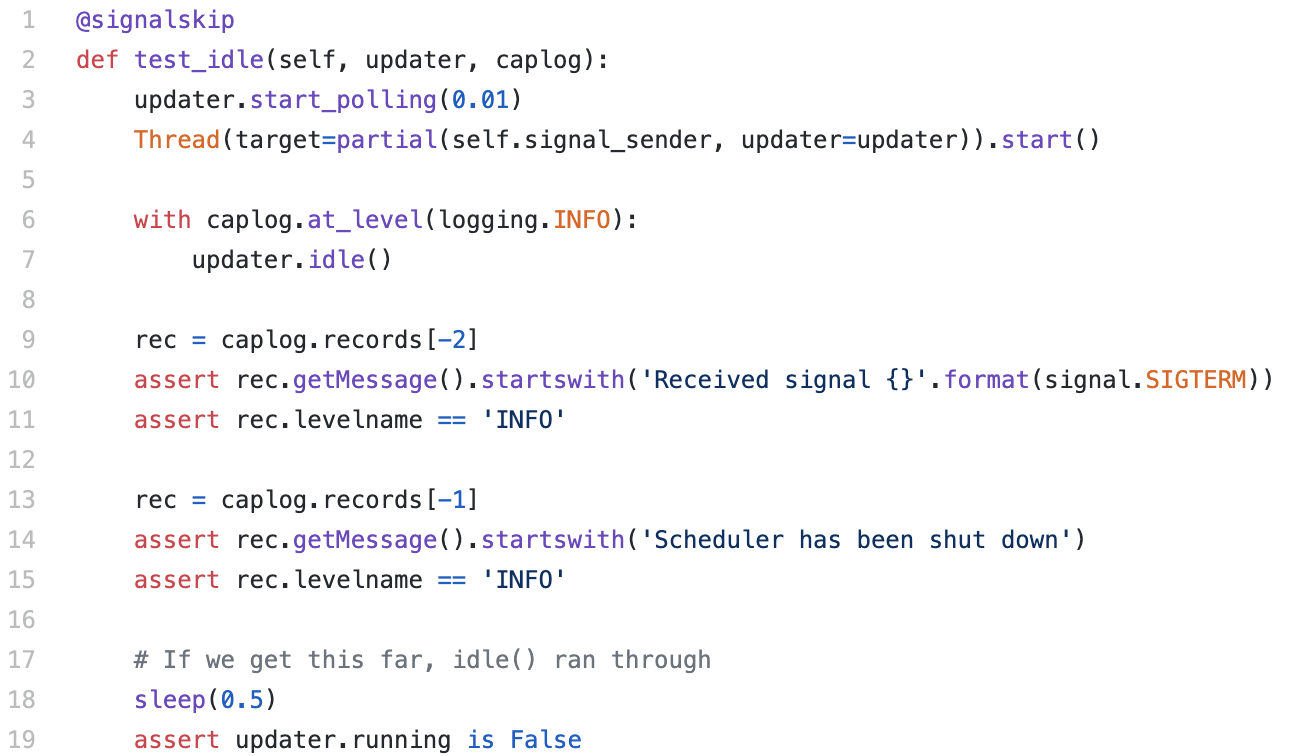
\includegraphics[width=0.8\textwidth]{figures/replication/manifestFlakyExample.png}
\caption{A manifest flaky test not labelled @flaky}
\label{manifest-flaky-example}
\end{figure}

Figure \ref{manifest-flaky-example2} shows the test \texttt{test\_to\_dict()} from the class \texttt{TestStickerSet}, which is also manifestly flaky but the developers did not mark it as such. 
Unordered collections have been identified as a cause of flakiness by several works as developers can wrongly assume that elements of a collection will be returned in a specific order~\cite{Luo2014,Dutta2020}.
In Python, the return order of dictionaries has varied over the different versions~\cite{PythonDoc, unorderedCollectionsStackOverflow}. In our case, we found that the keyword \texttt{dict}, which is present in a large number in this test, was among the first eight most important features of our classifier.
This feature allowed the vocabulary-based model to predict that this test is flaky.

\begin{figure}[ht]
\centering
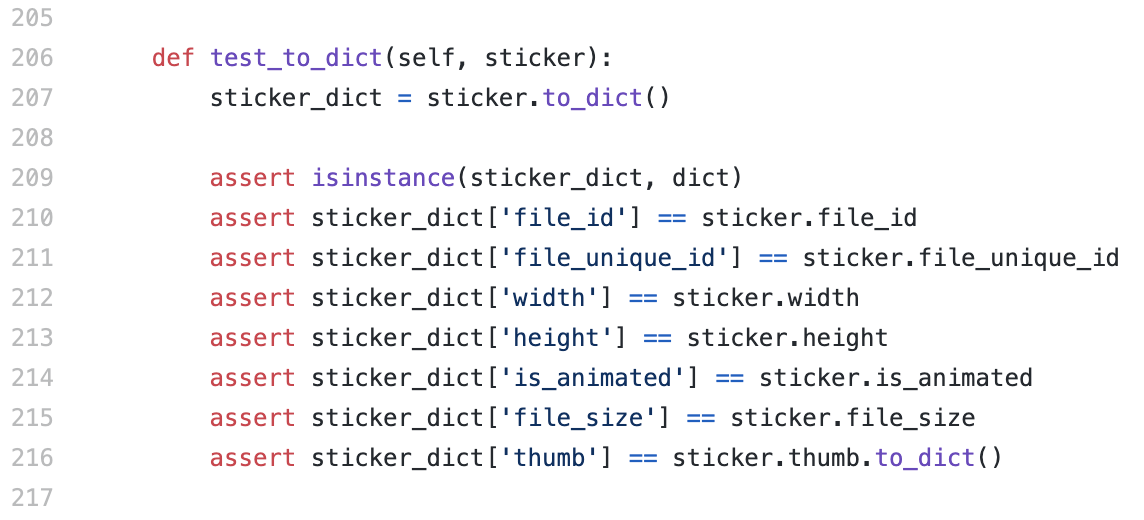
\includegraphics[width=0.8\textwidth]{figures/replication/manifestFlakyExample2.png}
\caption{A manifest flaky test not labelled @flaky}
\label{manifest-flaky-example2}
\end{figure}

We conclude that the approach is extendable to the Python language, supporting the idea that the vocabulary-based prediction can be generalisable to other projects and programming languages. Moreover, we saw that we can take advantage of a flaky tests classifier using vocabulary-based features in order to identify vocabulary linked to flakiness and help developers write better quality tests.\\

\begin{tcolorbox}[
    left=2pt,right=2pt,top=2pt,bottom=2pt,
    arc=0pt,
    boxrule=1.2pt
]
\textbf{RQ2:} Vocabulary-based models can be generalised to other projects and programming languages. 
Besides, these models can leverage annotated flaky tests to predict and annotate manifest flaky tests that were not known to developers.
\end{tcolorbox}

\subsection{RQ3: Extended Set of Features}

Figures~\ref{fig:prec-java-cut}-\ref{fig:mcc-java-cut} show the results of our prediction model in Java projects, while figures \ref{fig:prec-python-cut}-\ref{fig:mcc-python-cut} present the model performance in Python projects. 

\begin{figure}[!htbp]
  \centering
  \begin{minipage}[b]{0.4\textwidth}
    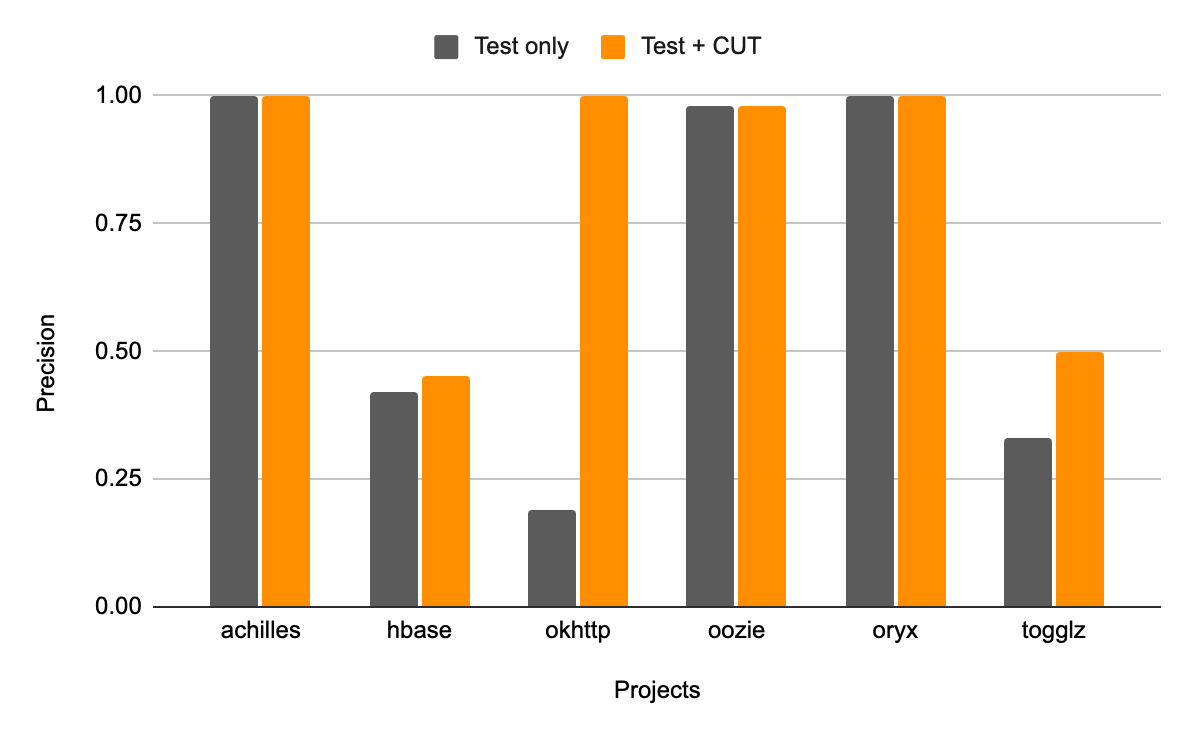
\includegraphics[width=\textwidth]{figures/replication/RQ3JavaPrecision.png}
    \caption{Precision score in Java projects}
    \label{fig:prec-java-cut}
  \end{minipage}
  \hfill
  \begin{minipage}[b]{0.4\textwidth}
    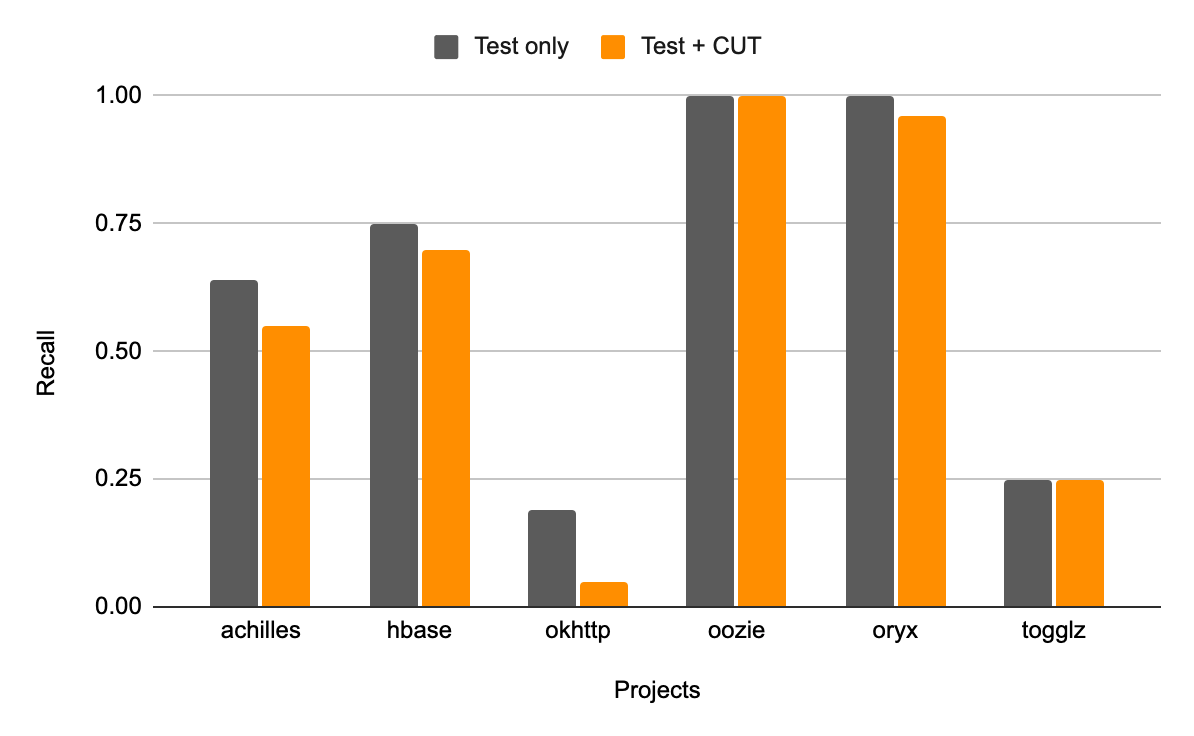
\includegraphics[width=\textwidth]{figures/replication/RQ3JavaRecall.png}
    \caption{Recall score in Java projects}
    \label{fig:recall-java-cut}
  \end{minipage}
  \hfill
  \begin{minipage}[b]{0.4\textwidth}
    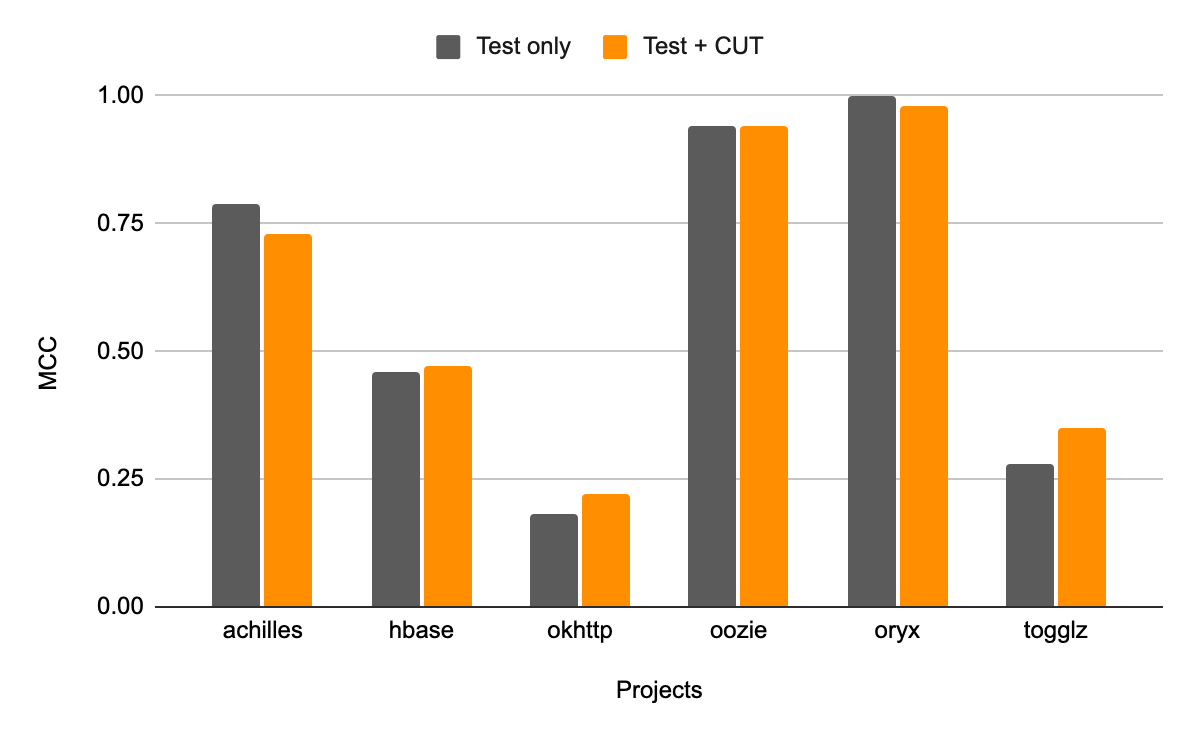
\includegraphics[width=\textwidth]{figures/replication/RQ3JavaMCC.png}
    \caption{MCC score in Java projects}
    \label{fig:mcc-java-cut}
  \end{minipage}
\end{figure}
\begin{figure}[!tbp]
  \centering
  \begin{minipage}[b]{0.4\textwidth}
    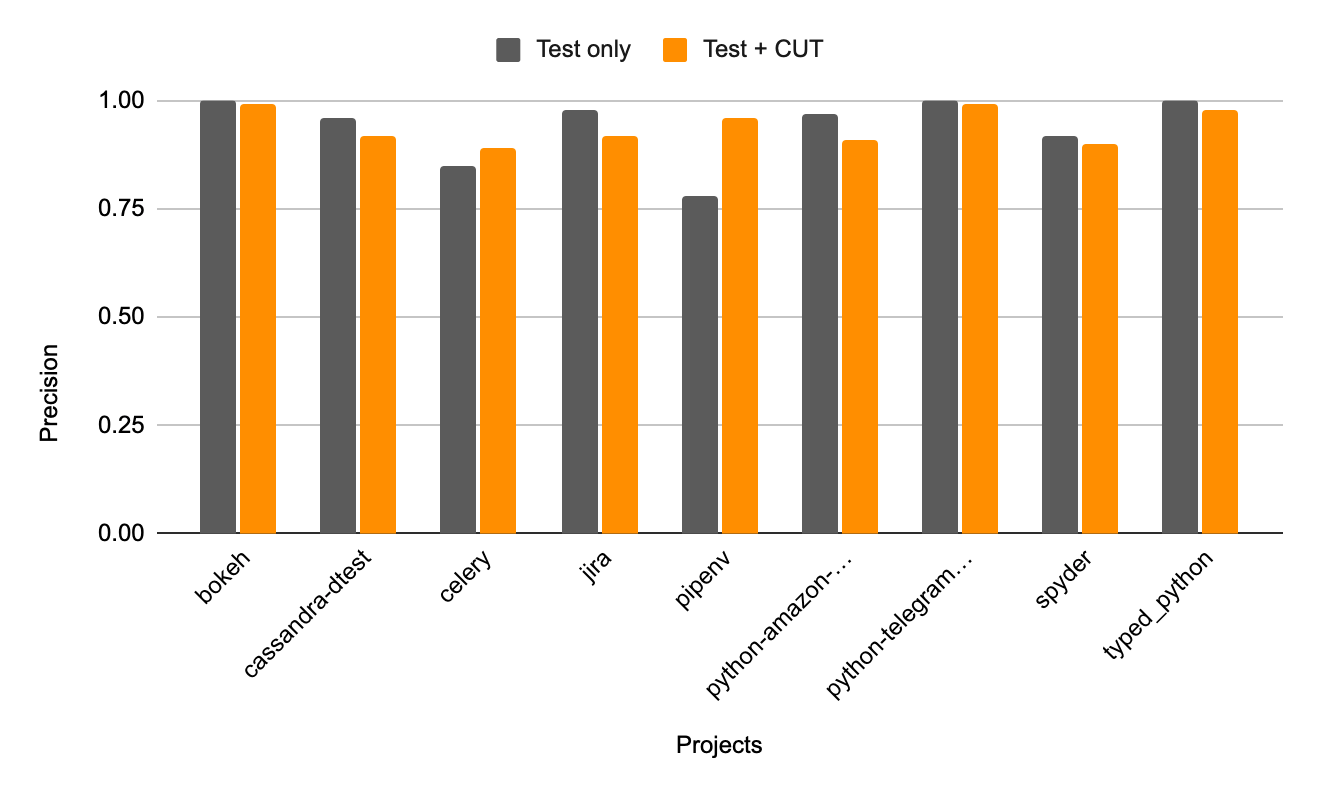
\includegraphics[width=\textwidth]{figures/replication/RQ3PythonPrecision.png}
    \caption{Precision score in Python projects}
    \label{fig:prec-python-cut}
  \end{minipage}
  \hfill
  \begin{minipage}[b]{0.4\textwidth}
    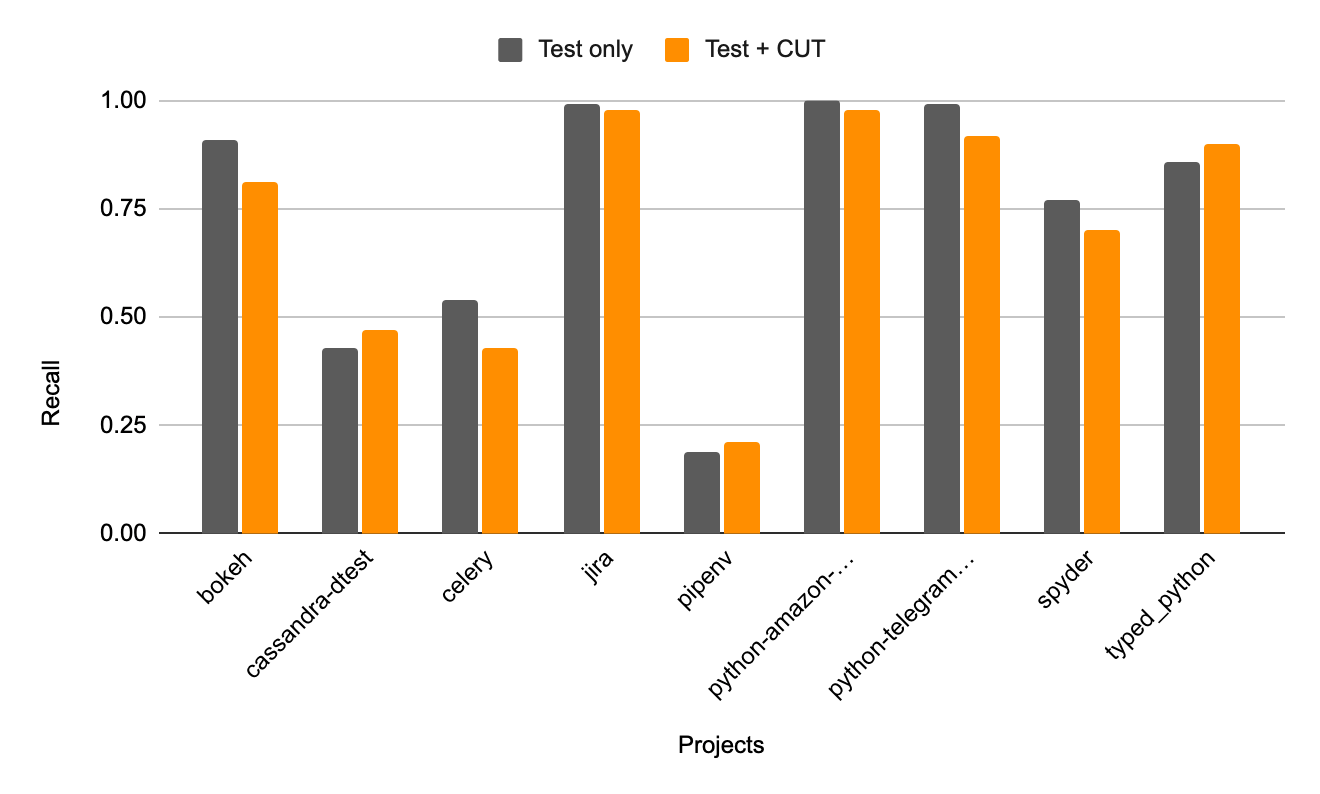
\includegraphics[width=\textwidth]{figures/replication/RQ3PythonRecall.png}
    \caption{Recall score in Python projects}
    \label{fig:rec-python-cut}
  \end{minipage}
  \hfill
  \begin{minipage}[b]{0.4\textwidth}
    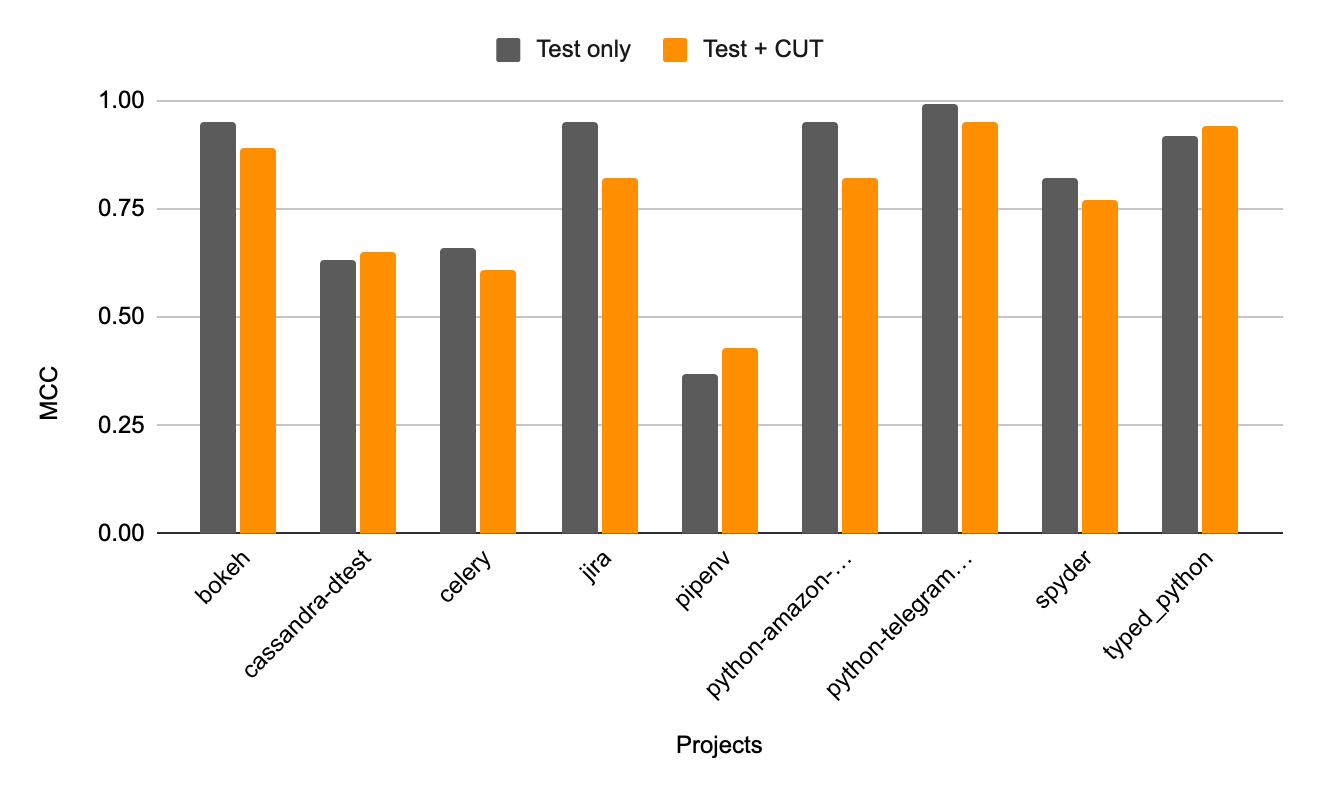
\includegraphics[width=\textwidth]{figures/replication/RQ3PythonMCC.png}
    \caption{MCC score in Python projects}
    \label{fig:mcc-python-cut}
  \end{minipage}
\end{figure}


In figures~\ref{fig:prec-java-cut}-\ref{fig:mcc-java-cut}, we observe that the impact of including the CUT does not have a consistent impact on the model performance in Java projects.
Adding the CUT improves the model performance in Hbase, Okhttp and Togglz, with an increase of the MCC value between 0.01 and 0.07.
However, the opposite effect is observed in the projects Achilles and Oryx where the MCC dropped by 0.06 and 0.02 respectively.
As for the Oozie project, including the CUT does not seem to impact the model performance.
Nonetheless, these performance improvements and losses remain minor in all the studied Java projects.

Figures \ref{fig:prec-python-cut}-\ref{fig:mcc-python-cut} show a similar effect of the CUT usage in Python projects.
Out of the nine studied, six projects report a lower performance when adding the CUT to the features.
This performance loss is up to 0.13 (MCC) in the projects Jira and Python-amazon.
On the other hand, the projects Cassandra-dtest, Pipenv, and Typed\_python have better predictions when the CUT is used --- an increase in the MCC value by 0.02, 0.06 and 0.02 respectively.

Based on the observations in both Java and Python, we conclude that including the CUT does not consistently improve the performance of a vocabulary-based model for predicting flaky tests.

\begin{tcolorbox}[
    left=2pt,right=2pt,top=2pt,bottom=2pt,
    arc=0pt,
    boxrule=1.2pt
]
\textbf{RQ3:} Surprisingly, the vocabulary of the Code Under Test, which is commonly considered as a source of flakiness, does not improve the performance of flakiness prediction models. 
\end{tcolorbox}
